% =====================================================================
% 附录 AM《磁体与超导：从临界电流到失超保护》
% 数值唯一来源：tools/calc/appAM_calc.py -> tools/calc/appAM_calc.txt（正文数字只引用该输出；检查项 P45）
% 单位写法：数字与单位都进数学模式；单位里带中文时用 \text{}（如 \text{匝}）
% 分级：现算级（脚本可复算）/ 声明级（脚本顶部输入，正文标明）/ 文献级（只作对照）
% 版权口径：只借鉴结论、公式形式与题型；文字、数值、表格自拟并独立复算；
%           本书不列 DOI，只给书名/作者/年份/卷期页
% 与相邻附录的分工：Z 讲堆的工程账与电厂、AG 讲平衡与位形、V 讲破裂的电磁载荷、
%           AB/AF 讲输运；本附录只补「环向场那台机器本身」——临界面、导体、
%           洛伦兹力、失超保护与制冷电耗
% =====================================================================

\section{为什么必须超导：一张电费单}
\label{sec:app-am-sc}

附录 Z 算过一座聚变堆的功率账，附录 AG 算过平衡与位形，
但它们都默认了一件事：\textbf{环向场是白来的}。
真实装置里，$5.3\ \mathrm{T}$ 的环向场要么由铜线圈通电流产生，要么由超导线圈产生。
这两条路的差别不在物理，在\textbf{电费单}。

先从设计的第一个方程开始。环向场沿大半径近似按 $1/R$ 衰减，
把安培环路定理用在半径 $R_0$ 处，得到\textbf{安培匝数}：

\begin{equation}
NI=\frac{2\pi R_0B_{TF}}{\mu_0}
=\frac{2\pi\times6.2\times5.3}{1.2566370614\times10^{-6}}
=1.643\times10^{8},
\label{eq:app-am-ampere}
\end{equation}

也就是 $1.643\times10^{8}$ 安培匝。若导体取 $68.0\ \mathrm{kA}$（ITER 量级），
每个线圈要 $134.232$ 匝，18 个线圈一共 $121.45\ \mathrm{km}$ 导体。
这个长度是后面所有账目的公共因子：\textbf{磁体的成本、损耗、力与储能都与它成正比}。

铜方案的电流密度受水冷限制，取 $5\ \mathrm{A\,mm^{-2}}$，
导体截面 $1.36\times10^{-2}\ \mathrm{m^{2}}$，总电阻 $0.151813\ \Omega$，
于是稳态电耗

\begin{equation}
P_{Cu}=I^{2}R_{Cu}
=(68.0\times10^{3})^{2}\times0.151813
=7.01983\times10^{8}\ \mathrm{W}
=701.983\ \mathrm{MW}.
\label{eq:app-am-pcu}
\end{equation}

把它和附录 Z 的聚变功率放在一起：$701.983/556.5=1.26142$。
\textbf{铜磁体自己就要吃掉 1.26 倍的聚变功率}——电厂还没发电就已经亏本了。
这不是工程细节，而是「聚变堆为什么必须用超导」的第一性回答。

超导方案的电耗不来自焦耳热，而来自制冷。把 $5\ \mathrm{kW}$ 的热量从
$4.5\ \mathrm{K}$ 抽到 $300\ \mathrm{K}$，理想卡诺循环要做的功是

\begin{equation}
W_{carnot}=Q\left(\frac{T_{h}}{T_{c}}-1\right)
=5.0\times10^{3}\times\left(\frac{300}{4.5}-1\right)
=3.28333\times10^{5}\ \mathrm{W},
\label{eq:app-am-carnot}
\end{equation}

按相对卡诺效率 $25\%$ 折算，制冷电耗 $1.31333\times10^{6}\ \mathrm{W}=1313.33\ \mathrm{kW}$。
两条路的比值是 $534.505$——\textbf{同一套安培匝数，电费差五百多倍}。
记住这个数字，它解释了为什么全世界的托卡马克从 1980 年代起都换成超导磁体。

\begin{table}[htbp]
\centering
\small
\begin{tabular}{p{3.5cm}p{3.6cm}p{3.4cm}p{3.6cm}}
\toprule
量 & 铜方案（$5\ \mathrm{A\,mm^{-2}}$） & 超导方案 & 说明 \\
\midrule
安培匝数 & $1.643\times10^{8}$ & $1.643\times10^{8}$ & 由 $B_{TF}$ 定，与材料无关 \\
导体截面 & $1.36\times10^{-2}\ \mathrm{m^{2}}$ & $1.7\times10^{-3}\ \mathrm{m^{2}}$ & 超导可承受 $40\ \mathrm{A\,mm^{-2}}$ \\
总长 & $121.45\ \mathrm{km}$ & $121.45\ \mathrm{km}$ & 同一个几何 \\
稳态电耗 & $701.983\ \mathrm{MW}$ & $1313.33\ \mathrm{kW}$ & 铜烧焦耳热，超导烧制冷功 \\
与 $P_{fus}$ 之比 & $1.26142$ & $2.35999\times10^{-3}$ & 铜方案直接出局 \\
\bottomrule
\end{tabular}
\caption{同一套安培匝数的两条路：铜的电耗是聚变功率的 $1.26$ 倍，超导的制冷电耗只有千分之二（数值唯一来源 \texttt{tools/\allowbreak{}calc/\allowbreak{}appAM\_calc.py}）。}
\label{tab:app-am-sc}
\end{table}

\begin{tip}{超导不是为了「更强」，是为了「不烧电」}{tip-app-am-why}
超导磁体并不比铜磁体产生更强的场——同样 $5.3\ \mathrm{T}$ 只需要同样的安培匝数。
它换掉的是损耗通道：铜把电变成热，超导把热从冷端搬到热端。
所以超导磁体的设计目标不是「电流更大」，而是\textbf{让每一瓦漏进冷端的功率都尽可能小}。
这是本附录后半部分（失超保护、制冷、交流损耗）全部内容的出发点。
\end{tip}

{\footnotesize
\textbf{出处：}磁体设计方程与超导磁体的工程口径参照 Wilson \emph{Superconducting Magnets}（1983，第 1--2 章）。
Iwasa \emph{Case Studies in Superconducting Magnets}（第 2 版，2009，第 1--3 章）。
Freidberg \emph{Plasma Physics and Fusion Energy}（2007，线圈与力章节）。
托卡马克环向场线圈的工程参数对照 ITER Physics Basis（\emph{Nuclear Fusion} 39，1999，第 1 章）。
}

\section{临界面：临界电流、温度裕度和 n 值}
\label{sec:app-am-critical}

超导体没有「电阻为零」这条绝对性质，只有\textbf{在某个区域内}电阻为零。
这个区域的边界是三个坐标的函数：磁场 $B$、温度 $T$、应变 $\varepsilon$。
工程上把它压成一条曲线：\textbf{临界电流密度} $J_c(B,T)$。

本书不引入实验拟合表，只用一个可以手算的\textbf{参数化}（声明级模型）：

\begin{equation}
J_c(B)=J_{c0}\left(1-\frac{B}{B_{c2}}\right)^{\beta},
\qquad J_{c0}=6000\ \mathrm{A\,mm^{-2}},\quad B_{c2}=26\ \mathrm{T},\quad \beta=1.5.
\label{eq:app-am-jc}
\end{equation}

代入三个典型场值：$J_c(5.3\ \mathrm{T})=4.26233\times10^{9}\ \mathrm{A\,m^{-2}}=4262.33\ \mathrm{A\,mm^{-2}}$、
$J_c(12\ \mathrm{T})=2370.74\ \mathrm{A\,mm^{-2}}$、
$J_c(20\ \mathrm{T})=665.148\ \mathrm{A\,mm^{-2}}$。
注意 $20\ \mathrm{T}$ 处已经掉到 $5.3\ \mathrm{T}$ 的 $1/6$——
\textbf{超导体的「强」是有条件的，条件就是场不能太高}。

导体的临界电流由临界电流密度乘上超导面积得到：

\begin{equation}
I_{c}=J_c\,A_{cab}\,f_{noncu}
=4.26233\times10^{9}\times1.7\times10^{-3}\times0.40
=2.89838\times10^{6}\ \mathrm{A}=2.89838\ \mathrm{MA}.
\label{eq:app-am-ic}
\end{equation}

工作电流只有 $68.0\ \mathrm{kA}$，于是 $I/I_c=0.0234614$——
本工作点的导体裕度有四十多倍。这个「宽裕」是假象：
真实装置的瓶颈在内腿（$12\ \mathrm{T}$ 以上）与应变退化，
本节把它单独列成一行，正是为了说明\textbf{裕度必须按最坏的那一点算}。

温度这一维同样要算。临界温度随场下降，用一个简化的
$T_c(B)=T_{c0}\sqrt{1-B/B_{c2}}$（$T_{c0}=18.0\ \mathrm{K}$）：
$T_c(5.3\ \mathrm{T})=16.0609\ \mathrm{K}$、$T_c(12\ \mathrm{T})=13.2084\ \mathrm{K}$。
把工作电流对应的\textbf{分流温度} $T_{cs}$ 解出来（工作点落在 $J_c$ 曲线的几分之一处）：

\begin{equation}
T_{cs}=T_c-\left(T_c-T_{op}\right)\frac{J_{op}^{noncu}}{J_c}
=16.0609-\left(16.0609-4.5\right)\times\frac{1.0\times10^{8}}{4.26233\times10^{9}}
=15.7897\ \mathrm{K},
\label{eq:app-am-tcs}
\end{equation}

温度裕度 $T_{cs}-T_{op}=11.2897\ \mathrm{K}$。
真实装置的温度裕度设计值只有 $1.5$--$2\ \mathrm{K}$——
差距来自应变退化与内腿的 $12\ \mathrm{T}$，也来自一个事实：
\textbf{温度裕度是设计出来的，不是算出来的}，算出来的只是它的上界。

\begin{table}[htbp]
\centering
\small
\begin{tabular}{p{2.6cm}p{3.4cm}p{3.2cm}p{3.2cm}}
\toprule
磁场 & 临界电流密度 & 电缆临界电流 & 工作点比值 $I/I_c$ \\
\midrule
$5.3\ \mathrm{T}$ & $4262.33\ \mathrm{A\,mm^{-2}}$ & $2.89838\ \mathrm{MA}$ & $0.0234614$ \\
$12\ \mathrm{T}$ & $2370.74\ \mathrm{A\,mm^{-2}}$ & $1.6121\ \mathrm{MA}$ & $0.042181$ \\
$20\ \mathrm{T}$ & $665.148\ \mathrm{A\,mm^{-2}}$ & $0.4523\ \mathrm{MA}$ & $0.150343$ \\
\bottomrule
\end{tabular}
\caption{临界面上的三个点：场越高，可用的电流密度越小，工作点被迫向 $I_c$ 靠近（$I_c$ 按电缆 $1700\ \mathrm{mm^{2}}$、非铜份额 $0.40$ 折算）。}
\label{tab:app-am-critical}
\end{table}

超导体的伏安特性不是阶跃，而是一条幂律：

\begin{equation}
E=E_0\left(\frac{I}{I_c}\right)^{n},
\qquad n\approx20,
\label{eq:app-am-nvalue}
\end{equation}

本工作点 $I/I_c=0.0234614$，电压只有基准的 $2.55308\times10^{-33}$ 倍——
\textbf{n 值把「接近临界」变成了一个极陡的开关}，
这正是失超检测能用电压信号抓住扰动的原因。

\begin{tip}{裕度是三个坐标上的距离，不是一个数}{tip-app-am-margin}
$J_c$、$T_c$、$I_c$ 三个名字容易让人以为超导体只有一个余量。
实际设计中它们是一组联立约束：场升高会同时拉低 $J_c$ 与 $T_c$，
应变退化再在两者之上乘一个因子。
所以「这个导体够不够用」永远要写成\textbf{在 $(B,T,\varepsilon)$ 空间里还有多远}，
而不是「离临界电流还有几安培」。
\end{tip}

{\footnotesize
\textbf{出处：}超导临界面的参数化与 $n$ 值口径参照 Wilson \emph{Superconducting Magnets}（1983，第 3--5 章）。
Bottura 与 Godeke \emph{Reviews of Accelerator Science and Technology} 5（2012，超导材料与导体综述）。
Iwasa（2009，第 4--5 章）。
$12\ \mathrm{T}$ 与应变退化的工程口径对照 Mitchell 等 \emph{IEEE Transactions on Applied Superconductivity} 21（2011，ITER 磁体）。
}

\begin{figure}[htbp]
\centering
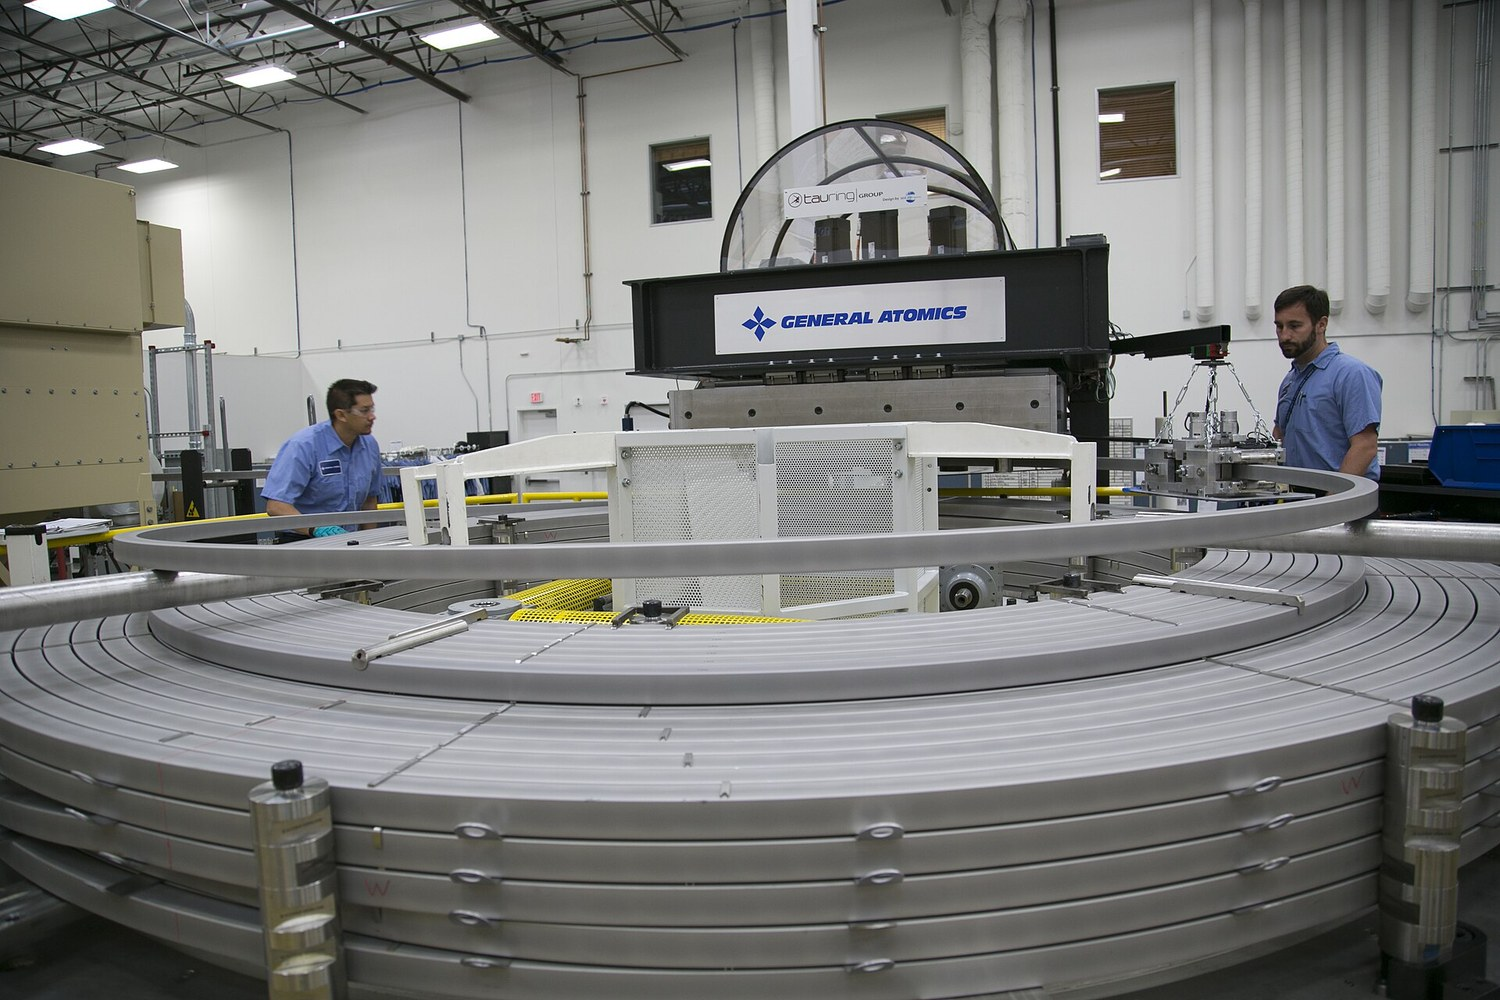
\includegraphics[width=0.72\textwidth]{../figures/am_iter_solenoid.jpg}
\caption{等离子体电流不是凭空来的：中心螺线管就是变压器的原边，等离子体是它的副边。本节讲 CICC 导体与氦冷，图中就是这种导体被绕成巨型线圈的现场。}
\label{fig:photo-appam2}
\figsource{Oak Ridge National Laboratory，CC BY 2.0（Wikimedia Commons）}
\end{figure}

\section{导体与 CICC：为什么电缆要泡在氦里}
\label{sec:app-am-cicc}

$68.0\ \mathrm{kA}$ 这样的电流不可能用一根超导丝承担。
工程上的做法是把上千根细丝拧成\textbf{电缆}，再套进一根不锈钢\textbf{导管}，
让超临界氦在导管里流过——这就是 CICC（cable-in-conduit conductor）。
本节的账只有三个数：电缆截面、铜的份额、以及\textbf{稳定化判据}。

电缆截面由工作电流与平均电流密度定：$A_{cab}=68.0\times10^{3}/40=1.7\times10^{-3}\ \mathrm{m^{2}}=1700\ \mathrm{mm^{2}}$。
其中铜占 $60\%$，超导占 $40\%$：超导部分承担 $1.0\times10^{8}\ \mathrm{A\,m^{-2}}$，
铜部分在分流后承担 $66.6667\ \mathrm{A\,mm^{-2}}$。
铜不是「杂质」，它是\textbf{分流通道}——扰动来临时电流有地方可去。

稳定性用最经典的 Stekly 判据检验：铜的焦耳热必须小于冷媒能带走的换热。
取冷态铜电阻率 $1.0\times10^{-9}\ \Omega\,\mathrm{m}$、卡皮查换热系数 $1000\ \mathrm{W\,m^{-2}\,K^{-1}}$、
受热周长 $0.20\ \mathrm{m}$、允许温升 $1.0\ \mathrm{K}$：

\begin{equation}
I_{stekly}=\sqrt{\frac{h\,P\,\Delta T}{\rho_{Cu}/A_{Cu}}}
=\sqrt{\frac{200}{9.80392\times10^{-7}}}
=14282.9\ \mathrm{A}=14.2829\ \mathrm{kA}.
\label{eq:app-am-stekly}
\end{equation}

工作电流 $68.0\ \mathrm{kA}$ 对应 $\alpha=22.6667$，也就是\textbf{超出池沸腾冷却能力二十多倍}。
结论不是「CICC 不稳定」，而是\textbf{池沸腾判据在这里根本用不上}：
CICC 靠的不是表面换热，而是导管里氦的\textbf{焓}——
把整段氦升温 $1$--$2\ \mathrm{K}$ 所能吸收的能量，比表面换热大几个量级。
这就是为什么聚变磁体的冷却是\textbf{强制流}而不是泡在液氦里。

\begin{table}[htbp]
\centering
\small
\begin{tabular}{p{3.4cm}p{3.3cm}p{3.6cm}p{3.6cm}}
\toprule
量 & 数值 & 口径 & 说明 \\
\midrule
电缆截面 & $1700\ \mathrm{mm^{2}}$ & $I/J_{op}$ & $40\ \mathrm{A\,mm^{-2}}$ \\
铜截面 & $1020\ \mathrm{mm^{2}}$ & $60\%$ & 分流通道 \\
单位长度电阻 & $9.80392\times10^{-7}\ \Omega\,\mathrm{m^{-1}}$ & 冷态电阻率 & 失超时的主要热源 \\
单位长度换热 & $200\ \mathrm{W\,m^{-1}}$ & $1\ \mathrm{K}$ 温升 & 池沸腾上界 \\
Stekly 电流 & $14.2829\ \mathrm{kA}$ & 判据 & 只到工作电流的 $1/5$ \\
\bottomrule
\end{tabular}
\caption{CICC 的三个数：截面、铜份额、稳定化电流。Stekly 判据在这里失效，恰好说明了强制流氦的必要性。}
\label{tab:app-am-cicc}
\end{table}

\begin{tip}{铜不是「拖累」，是失超时的救生通道}{tip-app-am-cicc}
超导电缆里最反直觉的一条设计原则是：\textbf{故意掺进大量铜}。
正常运行时它只占体积、不加分；一旦局部扰动把超导推过临界，
电流必须立刻有一条低电阻的路可走，否则能量会在几毫米内变成热点。
铜的份额、电阻率与冷却方式共同决定了导体能承受多大的扰动——
这三者合起来才是「稳定性」的定义。
\end{tip}

\textbf{出处：}CICC 与稳定化判据参照 Wilson（1983，第 6--8 章）。
Iwasa（2009，第 6--7 章）。
Bottura 与 Godeke（2012）。
强制流超临界氦的工程口径对照 Mitchell 等（2011）与 ITER Physics Basis（1999，第 1 章）。
\begin{figure}[htbp]
\centering
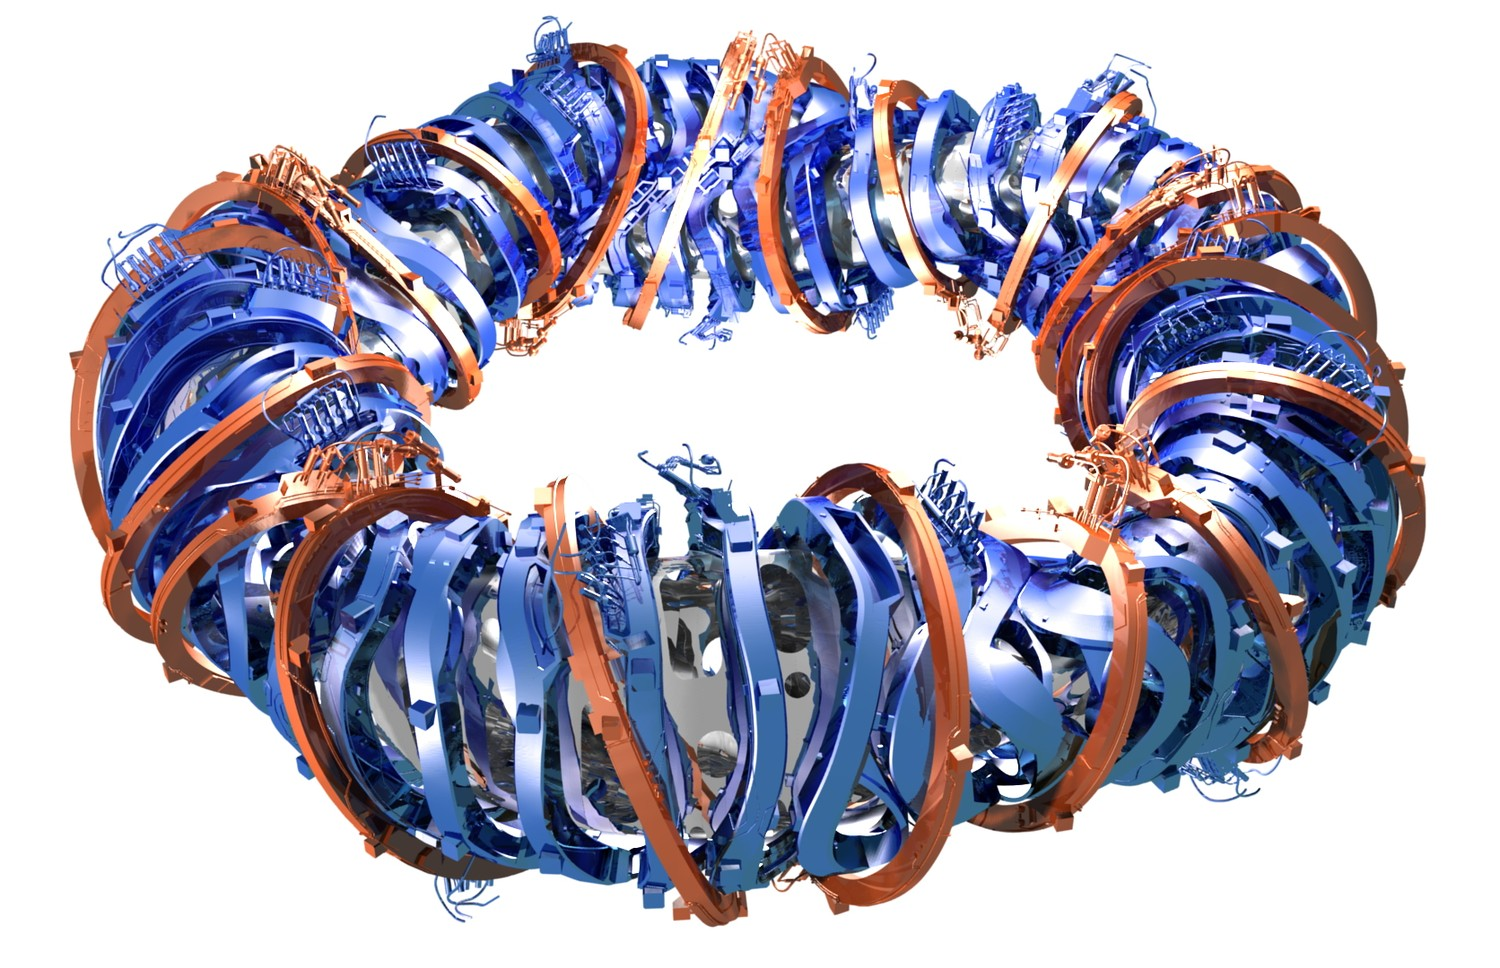
\includegraphics[width=0.72\textwidth]{../figures/w7x_magnets.jpg}
\caption{磁体系统长什么样：仿星器的线圈排布。这张示意图把「磁体首先是结构件」画在明处：每一根线圈都要同时满足临界电流、洛伦兹力与冷量三条约束，形状本身就是这些约束的解。}
\label{fig:photo-appam}
\figsource{M. Nagel, C.P. Dhard, H. Bau, H.-S. Bosch, U. Meyer, S. Raatz, K. Risse and T. Rummel，CC BY 3.0（Wikimedia Commons），链接见 figures/CREDITS.md。}
\end{figure}

\section{洛伦兹力与应力：磁体首先是结构件}
\label{sec:app-am-force}

超导体给出的是电流，电流与磁场的乘积给出的是\textbf{力}。
这个力不是副产品，它是磁体设计的\textbf{主载荷}——
一台聚变磁体首先是结构件，其次才是电学器件。

先看场本身的能量密度。附录 X 里出现过同一个数：
磁场压强

\begin{equation}
p_B=\frac{B^{2}}{2\mu_0}
=\frac{5.3^{2}}{2\times1.2566370614\times10^{-6}}
=1.11767\times10^{7}\ \mathrm{Pa}
=11.1767\ \mathrm{MPa}=111.767\ \mathrm{bar},
\label{eq:app-am-pb}
\end{equation}

也就是 $11$ 个大气压量级的\textbf{磁压}。它不是某个局部点的压强，
而是「磁场本身携带多少能量密度」的度量。

再看导体受到的线载荷。一段载流导体在磁场里受到单位长度力

\begin{equation}
f=IB_{TF}=68.0\times10^{3}\times5.3=3.604\times10^{5}\ \mathrm{N\,m^{-1}}
=360.4\ \mathrm{kN\,m^{-1}},
\label{eq:app-am-florentz}
\end{equation}

把它沿内腿（高度 $8.0\ \mathrm{m}$）对 $134.232$ 匝求和，
就是每个线圈承受的\textbf{向心（致心）力}：

\begin{equation}
F_{coil}=f\,h_{inner}N_{percoil}
=3.604\times10^{5}\times8.0\times134.232
=3.86349\times10^{8}\ \mathrm{N}=386.349\ \mathrm{MN},
\label{eq:app-am-hoop}
\end{equation}

18 个线圈合计 $6.95428\ \mathrm{GN}$。
$386.349\ \mathrm{MN}$ 是什么概念？它相当于把 $4$ 万吨的重物挂在第一个线圈上——
而且这台机器要求这个力在二十年里不把绝缘压坏、不把导体磨穿。

力最终要靠钢材承担。把力摊到绕组包截面 $0.456389\ \mathrm{m^{2}}$ 上：

\begin{equation}
\sigma=\frac{F_{coil}}{A_{wp}}
=\frac{3.86349\times10^{8}}{0.456389}
=8.46534\times10^{8}\ \mathrm{Pa}=846.534\ \mathrm{MPa}
=0.940594\,\sigma_{y},
\label{eq:app-am-stress}
\end{equation}

其中 $\sigma_y=900\ \mathrm{MPa}$ 是高强钢屈服强度的量级。
\textbf{平均应力已经用掉屈服强度的 $94\%$}，局部应力集中处必然超标——
这就是为什么线圈必须整体装进\textbf{钢盒}（case），
再由楔形支承把向心力传出去，而不是指望绕组自己扛。
把绕组包截面减半，应力立刻升到 $1693.07\ \mathrm{MPa}$：
\textbf{磁体的结构设计没有「差不多」这个选项}。

\begin{table}[htbp]
\centering
\small
\begin{tabular}{p{3.2cm}p{3.5cm}p{3.4cm}p{3.6cm}}
\toprule
量 & 表达式 & 数值 & 说明 \\
\midrule
磁压 & $B^{2}/2\mu_0$ & $11.1767\ \mathrm{MPa}$ & 能量密度口径 \\
单位长度力 & $IB$ & $360.4\ \mathrm{kN\,m^{-1}}$ & 导体上的载荷 \\
每线圈向心力 & $f h N$ & $386.349\ \mathrm{MN}$ & 内腿求和 \\
全部 18 个线圈 & $\times18$ & $6.95428\ \mathrm{GN}$ & 全机载荷 \\
平均应力 & $F/A_{wp}$ & $846.534\ \mathrm{MPa}$ & $0.940594\,\sigma_y$ \\
\bottomrule
\end{tabular}
\caption{力的传递链：磁压 $\to$ 线载荷 $\to$ 线圈向心力 $\to$ 截面应力。最后一行决定了线圈盒的材料与尺寸。}
\label{tab:app-am-force}
\end{table}

\begin{tip}{磁体是结构件，不是「绕线」}{tip-app-am-force}
初学者容易把磁体想成「把导线绕成圈，通电就行了」。
真实的设计顺序恰好相反：\textbf{先算力与应力，再决定导体与绝缘能放在哪里}。
同样的 $5.3\ \mathrm{T}$，在小装置上可以是铜线圈加支架，
在堆级尺度上必须是「钢盒 $+$ 楔形支承 $+$ 预应力」的组合结构。
力不只决定材料，还决定了装配顺序与检修方案。
\end{tip}

{\footnotesize
\textbf{出处：}磁压与洛伦兹力的口径参照 Wilson（1983，第 2 章）。
Freidberg \emph{Plasma Physics and Fusion Energy}（2007，线圈与力章节）。
Wesson \emph{Tokamaks}（第 4 版，2011，磁体与结构章节）。
线圈向心力量级对照 Mitchell 等（2011）与 ITER Physics Basis（1999，第 1 章）。
}

\section{失超与保护：能量必须有个出口}
\label{sec:app-am-quench}

超导磁体最危险的状态不是「没有电流」，而是\textbf{电流还在、超导却没了}。
这种状态叫失超（quench）。它的能量账必须先算清楚，
因为\textbf{能量不会消失，只会换一个地方变成热}。

先算储能。把场区等效成半径 $a_B=3.5\ \mathrm{m}$ 的环体，
体积 $V_B=2\pi R_0\cdot\pi a_B^{2}=1499.19\ \mathrm{m^{3}}$，
储能等于能量密度乘体积：

\begin{equation}
W=p_B\,V_B
=1.11767\times10^{7}\times1499.19
=1.6756\times10^{10}\ \mathrm{J}=16.756\ \mathrm{GJ}.
\label{eq:app-am-energy}
\end{equation}

$16.756\ \mathrm{GJ}$ 相当于 $4$ 吨 TNT 的能量。
它在正常运行时安静地存在磁场里，失超时必须\textbf{在几秒内被搬到磁体外面}。
由储能反推电感与泄能回路：

\begin{equation}
L=\frac{2W}{I^{2}}
=\frac{2\times1.6756\times10^{10}}{(68.0\times10^{3})^{2}}
=7.24739\ \mathrm{H},
\qquad
R_{dump}=\frac{L}{\tau}=0.724739\ \Omega,
\label{eq:app-am-inductance}
\end{equation}

取泄能时间常数 $\tau=10\ \mathrm{s}$，峰值电压 $I R_{dump}=49282.2\ \mathrm{V}=49.2822\ \mathrm{kV}$，
峰值功率 $I^{2}R_{dump}=3.35119\times10^{9}\ \mathrm{W}=3.35119\ \mathrm{GW}$。
\textbf{失超保护回路是一台 GW 级的脉冲功率设备}，它平时不工作，但必须随时可用。

能量最终变成热点温升。用绝热近似，铜里的积分 $\int J^{2}\mathrm{d}t$（常称 MIITs）决定温升：

\begin{equation}
\Delta T=\frac{\rho_{Cu}}{C_{Cu}}\int J^{2}\,\mathrm{d}t,
\qquad
\int J^{2}\,\mathrm{d}t=J_{Cu}^{2}\left(\tau_{detect}+\frac{\tau_{dump}}{2}\right),
\label{eq:app-am-miits}
\end{equation}

铜中电流密度 $J_{Cu}=66.6667\ \mathrm{A\,mm^{-2}}$，检测延迟 $1.0\ \mathrm{s}$，
于是正常保护下 $\int J^{2}\mathrm{d}t=2.66667\times10^{16}\ \mathrm{A^{2}\,s\,m^{-4}}$，

\begin{equation}
\Delta T=\frac{5.0\times10^{-9}}{1.5\times10^{6}}\times2.66667\times10^{16}
=88.8889\ \mathrm{K},
\label{eq:app-am-dt}
\end{equation}

冷端 $4.5\ \mathrm{K}$ 升到 $93.3889\ \mathrm{K}$，安全。
把允许温升定在 $150\ \mathrm{K}$，对应的上限是 $4.5\times10^{16}\ \mathrm{A^{2}\,s\,m^{-4}}$，
本设计用掉约六成——余量不到两倍。

如果保护失效（等效时间常数 $1000\ \mathrm{s}$），
$\int J^{2}\mathrm{d}t=2.22667\times10^{18}$，$\Delta T=7422.22\ \mathrm{K}$，
是允许值的 $49.4815$ 倍。\textbf{这个数字不是「更热一点」，是「导体已经变成等离子体」}。

\begin{table}[htbp]
\centering
\small
\begin{tabular}{p{3.2cm}p{4.0cm}p{3.2cm}p{3.3cm}}
\toprule
泄能时间常数 & $\int J^{2}\mathrm{d}t$ & 热点温升 & 判断 \\
\midrule
$5\ \mathrm{s}$ & 由上式 & $51.8519\ \mathrm{K}$ & 安全 \\
$10\ \mathrm{s}$ & $2.66667\times10^{16}$ & $88.8889\ \mathrm{K}$ & 安全（本设计） \\
$20\ \mathrm{s}$ & 由上式 & $162.963\ \mathrm{K}$ & 超过 $150\ \mathrm{K}$ 上限 \\
$1000\ \mathrm{s}$ & $2.22667\times10^{18}$ & $7422.22\ \mathrm{K}$ & 导体烧毁 \\
\bottomrule
\end{tabular}
\caption{保护时间常数决定一切：$10\ \mathrm{s}$ 与 $20\ \mathrm{s}$ 之间就跨过了 $150\ \mathrm{K}$ 的安全线。}
\label{tab:app-am-quench}
\end{table}

\begin{tip}{失超不是故障，是必须被设计进去的事件}{tip-app-am-quench}
「失超」听起来像事故，其实它是\textbf{保护策略的触发条件}：
检测到电压异常 $\to$ 切断电源 $\to$ 投入泄能电阻 $\to$ 把 $16.756\ \mathrm{GJ}$ 搬走。
真正的故障是\textbf{检测太慢}或\textbf{泄能回路失效}——
所以失超检测的响应时间、泄能电阻的可靠性、以及冷端的应急排放，
都是与磁体本体同等重要的设计内容。
\end{tip}

{\footnotesize
\textbf{出处：}储能、泄能与绝热热点模型参照 Wilson（1983，第 9--10 章）。
Iwasa（2009，第 8--9 章）。
Bottura 与 Godeke（2012）。
失超检测与保护的工程口径对照 Mitchell 等（2011）。
}

\section{制冷与交流损耗：冷量是最贵的电}
\label{sec:app-am-cryo}

超导磁体的电耗不在线圈里，而在\textbf{制冷机}里。
把热量从 $4.5\ \mathrm{K}$ 搬到 $300\ \mathrm{K}$ 需要付出的功由卡诺因子决定：

\begin{equation}
\mathrm{COP}^{-1}=\frac{T_{h}}{T_{c}}-1=\frac{300}{4.5}-1=66.6667,
\qquad
P_{cryo}=\frac{Q}{\eta_{carnot}}\left(\frac{T_{h}}{T_{c}}-1\right).
\label{eq:app-am-cop}
\end{equation}

取 $Q=5.0\ \mathrm{kW}$、$\eta_{carnot}=0.25$，得制冷电耗 $1.31333\times10^{6}\ \mathrm{W}=1313.33\ \mathrm{kW}$。
\textbf{冷端每漏进一瓦，电网要付二百多瓦}——所以磁体设计里
「少漏一点热」比「多一点裕度」更值钱。

第二笔冷负荷来自\textbf{交流损耗}。环向场在脉冲段要变化，
耦合电流在导体里产生损耗，其功率密度由耦合时间常数与场变化率决定：

\begin{equation}
q_{cpl}=\frac{n\tau}{\mu_0}\left(\frac{\mathrm{d}B}{\mathrm{d}t}\right)^{2}
=\frac{0.05}{1.2566370614\times10^{-6}}\times0.5^{2}
=9947.18\ \mathrm{W\,m^{-3}}.
\label{eq:app-am-coupling}
\end{equation}

绕组包体积 $412.931\ \mathrm{m^{3}}$，瞬时热负荷 $4.1075\times10^{6}\ \mathrm{W}=4.1075\ \mathrm{MW}$；
按 $10\ \mathrm{s}$ 斜坡折算，每次脉冲 $4.1075\times10^{7}\ \mathrm{J}=41.075\ \mathrm{MJ}$，
在 $1000\ \mathrm{s}$ 的脉冲周期里平均 $41075\ \mathrm{W}=41.075\ \mathrm{kW}$。
把它折算成制冷电耗是 $10.789\ \mathrm{MW}$——
\textbf{比稳态冷负荷的电耗（$1.31333\ \mathrm{MW}$）大八倍}。
脉冲装置的磁体设计，交流损耗往往才是主要矛盾。

\begin{table}[htbp]
\centering
\small
\begin{tabular}{p{3.6cm}p{3.4cm}p{3.4cm}p{3.3cm}}
\toprule
冷负荷项 & 热负荷 & 折算电耗 & 说明 \\
\midrule
稳态漏热（声明） & $5.0\ \mathrm{kW}$ & $1313.33\ \mathrm{kW}$ & 支撑、电流引线、辐射 \\
交流损耗（平均） & $41.075\ \mathrm{kW}$ & $10.789\ \mathrm{MW}$ & $\tau=0.05\ \mathrm{s}$、$\mathrm{d}B/\mathrm{d}t=0.5\ \mathrm{T\,s^{-1}}$ \\
合计 & --- & $12.1024\ \mathrm{MW}$ & 占 D-T 功率 $0.0217473$ \\
\bottomrule
\end{tabular}
\caption{制冷预算：同一条卡诺因子上，交流损耗把电耗从 $1.31333\ \mathrm{MW}$ 抬到 $12.1024\ \mathrm{MW}$。}
\label{tab:app-am-cryo}
\end{table}

\begin{tip}{冷量是最贵的电}{tip-app-am-cryo}
在 $4.5\ \mathrm{K}$ 上，$1\ \mathrm{W}$ 的热量要用 $200$--$300\ \mathrm{W}$ 的电去搬走。
这条换算把所有看起来「很小」的热源都放大成工程问题：
支撑漏热、电流引线、辐射、交流损耗、甚至测量线的铜损。
磁体设计里最常见的优化方向不是「提高临界电流」，
而是\textbf{把热负荷一项一项砍下来}。
\end{tip}

{\footnotesize
\textbf{出处：}制冷卡诺因子与交流损耗口径参照 Wilson（1983，第 8 章）。
Iwasa（2009，第 6 章）。
Bottura 与 Godeke（2012）。
耦合损耗时间常数的工程取值对照 Mitchell 等（2011）。
\section{估算练习}
\label{sec:app-am-problems}
}


\begin{enumerate}
\item \textbf{练习 1}：若把环向场从 $5.3\ \mathrm{T}$ 提到 $10.6\ \mathrm{T}$（几何不变），
储能与每个线圈的向心力各变多少倍？给出具体数值。
\item \textbf{练习 2}：铜磁体如果把允许电流密度从 $5\ \mathrm{A\,mm^{-2}}$ 放宽到 $10\ \mathrm{A\,mm^{-2}}$，
电耗变成多少？（导体总长 $121.45\ \mathrm{km}$、工作电流 $68.0\ \mathrm{kA}$、室温铜电阻率 $1.7\times10^{-8}\ \Omega\,\mathrm{m}$）
\item \textbf{练习 3}：泄能时间常数取 $5\ \mathrm{s}$、$10\ \mathrm{s}$、$20\ \mathrm{s}$ 三种情况，
热点温升分别是多少？哪一种越过 $150\ \mathrm{K}$ 的安全线？
（检测延迟 $1.0\ \mathrm{s}$、铜中电流密度 $66.6667\ \mathrm{A\,mm^{-2}}$、$\rho_{Cu}=5.0\times10^{-9}\ \Omega\,\mathrm{m}$、$C_{Cu}=1.5\times10^{6}\ \mathrm{J\,m^{-3}\,K^{-1}}$）
\item \textbf{练习 4}：若稳态冷负荷不是 $5.0\ \mathrm{kW}$ 而是 $20.0\ \mathrm{kW}$，
制冷电耗是多少？（卡诺因子按 $300/4.5$ 计算，相对卡诺效率 $0.25$）
\item \textbf{练习 5}：若临界电流密度因应变退化下降 $10\%$，工作点比值 $I/I_c$ 变成多少？
在同一条 $n=20$ 的幂律下，电压变成原来的几倍？
\item \textbf{练习 6}：若设计要求平均应力不超过 $540\ \mathrm{MPa}$，
绕组包截面至少要多大？与本书设计的 $0.456389\ \mathrm{m^{2}}$ 相比够不够？
\end{enumerate}

\textbf{解答 1}：储能 $\propto B^{2}$，$W=67.0239\ \mathrm{GJ}$，是原来的 $4$ 倍；
向心力 $\propto B$，$F=772.698\ \mathrm{MN}$，是原来的 $2$ 倍。
\textbf{场每翻一倍，储能的代价是四倍}——这是高场磁体设计最硬的一条约束。

\textbf{解答 2}：电流密度翻倍使导体截面减半、电阻翻倍，
电耗从 $0.701983\ \mathrm{GW}$ 升到 $1.40397\ \mathrm{GW}$。
也就是说「放宽电流密度」并不能救铜磁体，只会让它更快烧掉。

\textbf{解答 3}：$\Delta T$ 分别是 $51.8519\ \mathrm{K}$、$88.8889\ \mathrm{K}$、$162.963\ \mathrm{K}$。
$20\ \mathrm{s}$ 已经越过 $150\ \mathrm{K}$ 的安全线——\textbf{保护时间常数不是可以「差不多」的量}。

\textbf{解答 4}：$P_{cryo}=20.0\times10^{3}\times66.6667/0.25=5.25333\times10^{6}\ \mathrm{W}=5.25333\ \mathrm{MW}$。
冷负荷翻四倍，电耗也翻四倍；\textbf{冷端的账是线性的，所以每一项漏热都值得单独优化}。

\textbf{解答 5}：$I/I_c=0.0260682$，看起来仍然很小；
但在 $n=20$ 的幂律下电压升到原来的 $8.22526$ 倍。
\textbf{「离临界还很远」与「电压已经涨了八倍」可以同时成立}——
这就是超导磁体必须做电压监测的原因。

\textbf{解答 6}：$A_{wp}\ge F/540\ \mathrm{MPa}=0.715461\ \mathrm{m^{2}}$，
而本书设计只有 $0.456389\ \mathrm{m^{2}}$，\textbf{不够}。
要满足这条要求，绕组包必须加大约六成，或者改用屈服强度更高的钢。

\section{来源、分级与版权说明}
\label{sec:app-am-source}

\begingroup\small
本附录的数字分三级，读的时候请分清：

\textbf{现算级}：由 \texttt{tools/\allowbreak{}calc/\allowbreak{}appAM\_calc.py} 从声明量出发算出的量
（安培匝数、铜电耗、$J_c$、$I_c$、$T_{cs}$、$p_B$、向心力、应力、储能、$L$、$R_{dump}$、
$V_{peak}$、MIITs、$\Delta T$、卡诺因子、制冷电耗、耦合损耗）。

\textbf{声明级}：脚本顶部给定的输入——
$68.0\ \mathrm{kA}$、$40\ \mathrm{A\,mm^{-2}}$、非铜份额 $0.40$、填充因子 $0.50$、
$J_{c0}=6000\ \mathrm{A\,mm^{-2}}$、$B_{c2}=26\ \mathrm{T}$、$\beta=1.5$、
$T_{c0}=18.0\ \mathrm{K}$、$4.5\ \mathrm{K}$、相对卡诺效率 $0.25$、
$\tau_{dump}=10\ \mathrm{s}$、$\tau_{detect}=1.0\ \mathrm{s}$、
$C_{Cu}=1.5\times10^{6}\ \mathrm{J\,m^{-3}\,K^{-1}}$、$\rho_{Cu}=5.0\times10^{-9}\ \Omega\,\mathrm{m}$、
$n\tau=0.05\ \mathrm{s}$、$\mathrm{d}B/\mathrm{d}t=0.5\ \mathrm{T\,s^{-1}}$、$\eta_{carnot}=0.25$。
它们不是本书测出来的，而是从公开工程文献里取的量级；
换一组声明量，所有现算级数字都会按公式改变。

\textbf{文献级}：只用于对照的量级，例如「真实装置的温度裕度设计值 $1.5$--$2\ \mathrm{K}$」、
「内腿场强 $12\ \mathrm{T}$ 以上」、「$150\ \mathrm{K}$ 的失超温升上限」。
它们的作用是校准量级，不作为本附录的计算输入。

\begin{table}[htbp]
\centering
\small
\begin{tabular}{p{4.2cm}p{4.4cm}p{5.0cm}}
\toprule
来源 & 借鉴了什么 & 没有借鉴什么 \\
\midrule
Wilson \emph{Superconducting Magnets}（1983） & 安培匝数设计方程、稳定性判据、失超保护框架 & 图表、例题、具体装置参数 \\
Iwasa（2009，第 2 版） & 临界面的组织方式、CICC 的工程口径 & 原文文字、案例数据 \\
Bottura 与 Godeke（\emph{Rev. Accel. Sci. Tech.} 5，2012） & 超导材料与导体的综述框架 & 拟合系数与实验曲线 \\
Mitchell 等（\emph{IEEE Trans. Appl. Supercond.} 21，2011） & ITER 磁体的力量级与保护时间常数 & 工程设计图、材料牌号数据 \\
Freidberg（2007）、Wesson（2011） & 磁压与线圈受力的物理图像 & 习题与插图 \\
ITER Physics Basis（\emph{Nuclear Fusion} 39，1999） & 装置级参数的量级对照 & 表格与图 \\
\bottomrule
\end{tabular}
\caption{借鉴清单：只借鉴结论、公式形式与量级；所有数值、表格与题面由本书自拟并独立复算。}
\label{tab:app-am-source}
\end{table}

本附录的文字、公式推导、表格、题面与解答都是自拟的：
不复制上述文献的任何段落、图表或习题；
不复制文献里的拟合系数表，只保留可手算的参数化形式；
不复制任何装置的工程设计图与材料数据表；
不复制文献中对失超传播过程的原始描述，只保留本附录自己的绝热估算；
不复制各文献使用的符号体系，本附录的符号以本书附录 D 的符号表为准；
不声称本附录的参数化模型可以直接用于工程设计。

\begin{tip}{本附录不给什么}{tip-app-am-honest}
本附录给的是\textbf{量级模型}，不是磁体设计手册。它不给：
应变退化的定量标定、$J_c(B,T,\varepsilon)$ 的实验拟合、
失超传播速度与三维热传导、绝缘的辐照寿命、以及交流损耗的完整频谱模型。
它给的是这几件事的\textbf{入口}：
一台 $5.3\ \mathrm{T}$ 的磁体要多少安培匝、要吃掉多少电、
承受多大的力、储能往哪里去、冷端的每一瓦值多少电。
把这五笔账算清楚，再读任何一份磁体设计报告都不会迷路。
\end{tip}
\endgroup
